\documentclass{beamer}

\input{embed_video.tex}
\mode<presentation>
{
  \usetheme{Boadilla}
  % possiblities Singapore, Malmoe, Dresden 
  \setbeamercovered{invisible}
}

%\setbeamertemplate{navigation symbols}{} 
% removes the navigation symbols

%color setting more or less matching U of A colors
\setbeamercolor*{palette secondary}{use=structure,fg=white,bg=structure.fg!55!black}
\setbeamercolor*{palette tertiary}{use=structure,fg=white,bg=red!50!black}

\usepackage[english]{babel}
\usepackage{tikz}
\usetikzlibrary{patterns,hobby}
\usepackage{pgfplots}
\pgfplotsset{compat=1.6}
\usepgfplotslibrary{fillbetween}
\usepackage[utf8]{inputenc}
\usepackage[T1]{fontenc}
\usepackage{graphicx}
\usepackage{amsfonts}
\usepackage[
    backend=biber,
    style=phys,
    pageranges=false,
    biblabel=brackets,
    chaptertitle=false,
    articletitle=false,
    maxbibnames=3,
    doi=false, url=false, isbn=false
]{biblatex}
%\usepackage[backend=biber]{biblatex}
\addbibresource{presentation.bib}

\title[TPS free energies]{Transition path sampling and the calculation of free energies of enzymatic reactions}
%\subtitle{} 

\author[Schwartz Group]{Sree Ganesh Balasubramani}

\institute[U of A]{Schwartz Group \\ Chemistry and Biochemistry \\ University of Arizona}
\date{}

% If you wish to uncover everything in a step-wise fashion, uncomment
% the following command: 
%\beamerdefaultoverlayspecification{<+->}
\begin{document}
%------------------------------------------------------------------------------
\begin{frame}
  \titlepage
\end{frame}
%------------------------------------------------------------------------------
\begin{frame}
  \frametitle{Outline}
  \begin{itemize}[<+-|alert@+>]
      \item Motivations
      \item Introduction to transition path sampling 
      \item Equilibrium sampling within TPS
      \item Algorithm 
      \item Results
  \end{itemize}
\end{frame}
%------------------------------------------------------------------------------
\begin{frame}
\frametitle{Motivations}
\begin{block}{Why use molecular dynamics simulations?}
Understand enzyme activity in atomistic detail
\end{block}
\pause
\begin{block}{Why study enzyme activity?}
To help understand the design of inhibitors 
To design more efficient enzymes using directed evolution
\end{block}

\end{frame}
%------------------------------------------------------------------------------
\begin{frame}
\frametitle{Sampling rare but important events}
\begin{figure}
\centering
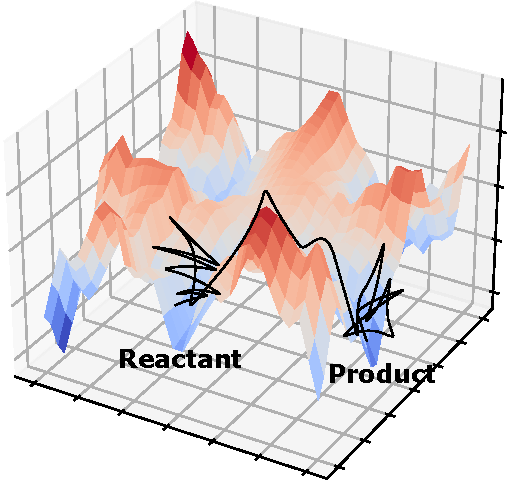
\includegraphics[scale=0.75]{figures/pot-surf.pdf}
\end{figure}
\end{frame}
%------------------------------------------------------------------------------
\begin{frame}
\frametitle{Transition path sampling (TPS)}
Transition path sampling is a rate event sampling method \footfullcite{Bolhuis02AnnRevPhysChem53p291}
that is free from bias
\end{frame}
%------------------------------------------------------------------------------
\begin{frame}
\frametitle{Trajectories in phase space}
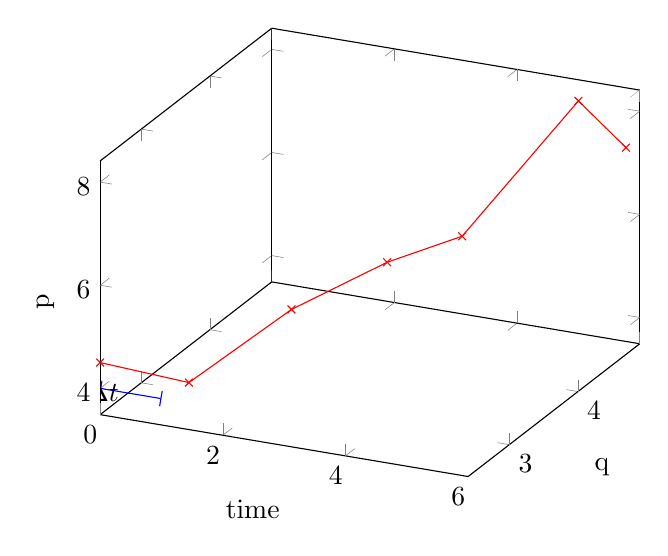
\begin{tikzpicture}
\begin{axis}[
    xlabel=time,
    ylabel=q,
    zlabel=p]
  \addplot3[color=red,mark=x] coordinates {
    (0.0,2.4,4.5)
    (1.0,2.8,3.9)
    (2.0,3.4,4.9)
    (3.0,3.9,5.5)
    (4.0,4.1,6.0)
    (5.0,4.9,8.0)
    (6.0,4.7,7.5)
  };
  \addplot3[color=blue,|-|] coordinates{ (0,2.4,4.0) (1,2.4,4.0)};
  \node[] at (1.5,2.0,.5) {$\Delta t$};
  \end{axis}
\end{tikzpicture}
\newline
The trajectory in phase space is defined by $x = \{\vec{q},\vec{p}\}$ where $\vec{q}$ 
is the generalized coordinates and $\vec{p}$ is the generalized momenta of the 
atoms in the system. 
\end{frame}
%------------------------------------------------------------------------------
\begin{frame}
\frametitle{Shooting algorithm}

\end{frame}
%------------------------------------------------------------------------------
\begin{frame}
\frametitle{TPS ensemble}
\begin{equation}
\mathcal{P}_{\mathcal{AB}}[z_{\mathcal{T}}] = h_{\mathcal{A}}(z_0)\mathcal{P}[z(\mathcal{T})]
h_{\mathcal{B}}(z_{\mathcal{T}})/Z_{\mathcal{AB}}(\mathcal{T})\label{eqn:tpsensem}
\end{equation}
where 
\[
    h_{\mathcal{A}/\mathcal{B}}(z)= 
\begin{cases}
    1, & \text{if } z\in \mathcal{A}/\mathcal{B}\\
    0,              & \text{otherwise}
\end{cases}
\]
and $Z_{\mathcal{AB}}(\mathcal{T})$ is the normalization factor for this 
probability distribution function.
\end{frame}
%------------------------------------------------------------------------------
\begin{frame}
\frametitle{Monte Carlo in path space}
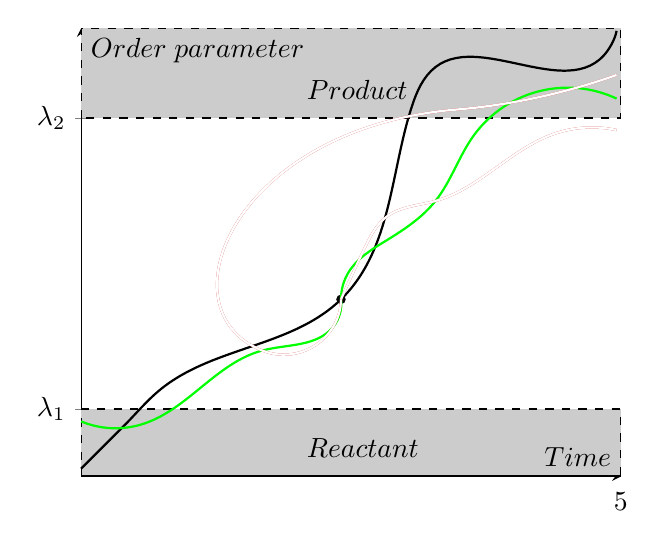
\begin{tikzpicture}
 \begin{axis}[
        xmin=0.0,xmax=5.0,
        ymin=0,ymax=5.0,
        xtick={0.0, 5.0},
        %xticklabels={$v_1$,$v_2$},
        ytick={0.75,4.0},
        yticklabels={$\lambda_1$,$\lambda_2$},
        xlabel={$Time$},  
        ylabel={$Order\;parameter$},
        every axis x label/.style={
    at={(ticklabel* cs:5.05)},
    anchor=west,
},
every axis y label/.style={
    at={(ticklabel* cs:5.05)},
    anchor=south,
},
        axis lines=middle] 
    \draw [fill=gray!40!white,thick,dashed] (axis cs:0,0) rectangle (axis cs:5.0,0.75);
    \draw [fill=gray!40!white,thick,dashed] (axis cs:0,4.0) rectangle (axis cs:5.0,5.0);
    \addplot+[black,thick,domain=0:5,no marks] {0};
    %
    \node  at (axis cs:2.0,4.1)    [anchor=south west] {$Product$};
    \node  at (axis cs:2.0,0.1)    [anchor=south west] {$Reactant$};
    \end{axis}
\pause
\draw [thick] (0.0 ,0.1) to [ curve through ={(0.5, 0.6) . . (0.55, 0.65)  . . (1.0,1.1) . . (3.3, 2.25) . . (4.2, 4.7) . . (4.5,5.2) . . (6.77, 5.56)  }] (6.8,5.66);% curve 
\pause
\filldraw (3.3,2.25) circle[radius=1.5pt];
\pause
\draw [green,thick] (3.3 ,2.25) to [ curve through ={(3.4,2.6)  . . (3.88, 3.00) . . (4.5,3.5) . . (5.0,4.35)  }] (6.8,4.8);% curve
\pause  
\draw [green,thick] (3.3 ,2.25) to [ curve through ={(3.2,1.9)  . . (2.3,1.6) . . (0.76,0.66)  }] (0.0,0.7);% curve 
\pause
\draw [gray!40!red,thick] (3.3 ,2.25) to [ curve through ={(3.6,2.9)  . . (3.88, 3.30) . . (4.5,3.5) . . (6.0,4.35)  }] (6.8,4.4);% curve
\pause  
\draw [gray!40!red,thick] (3.3 ,2.25) to [ curve through ={(3.2,1.9)  . . (2.3,1.6) . . (4.76,4.66)  }] (6.8,5.1);% curve 
\pause
\draw [white,thick] (3.3 ,2.25) to [ curve through ={(3.6,2.9)  . . (3.88, 3.30) . . (4.5,3.5) . . (6.0,4.35)  }] (6.8,4.4);% curve
\pause  
\draw [white,thick] (3.3 ,2.25) to [ curve through ={(3.2,1.9)  . . (2.3,1.6) . . (4.76,4.66)  }] (6.8,5.1);% curve 
\end{tikzpicture}
\end{frame}
%------------------------------------------------------------------------------
\begin{frame}
\frametitle{Equilibrium sampling in trajectory space}

\end{frame}
%------------------------------------------------------------------------------
\begin{frame}
\frametitle{The algorithm}

\end{frame}
%------------------------------------------------------------------------------
\begin{frame}
\frametitle{Free energies from TPS}
Window based sampling of order parameter

\begin{equation}
A[\zeta] = -k_BTlog(P(\zeta))
\end{equation}
\end{frame}
%------------------------------------------------------------------------------
\begin{frame}
\frametitle{QM/MM simulations}
CHARMM force field consists of intramolecular terms such as 
\begin{align}
E_{int} = &\sum_{bonds}k_r(r-r_{0})^2 + \sum_{angles}k_{\theta}(\theta - \theta_{0})^2 \nonumber \\ &+ \sum_{dihedrals}k_{\phi}(1+\cos(n\phi-\delta)) \nonumber \\
&+ \sum_{imp.\;dihed.} k_{\psi}(\psi - \psi_0)^2 + \sum_{Urey-Bradley} k_{\text{UB}}(r_{1,3}-r_{1,3;0}) \nonumber 
\end{align}\pause
and intermolecular terms such as 
\begin{align}
\sum_{nonbonded} \left(\frac{q_iq_j}{4\pi\epsilon r_{ij}} - E_{min} 
\left[\left(\frac{R_{min}}{r_{ij}}\right)^{12} - \left(\frac{R_{min}}{r_{ij}}\right)^{6} \right] \right)\nonumber 
\end{align}
\end{frame}
%------------------------------------------------------------------------------
\begin{frame}
\frametitle{Human adenosyl methionine enzyme}
\begin{figure}
\centering 
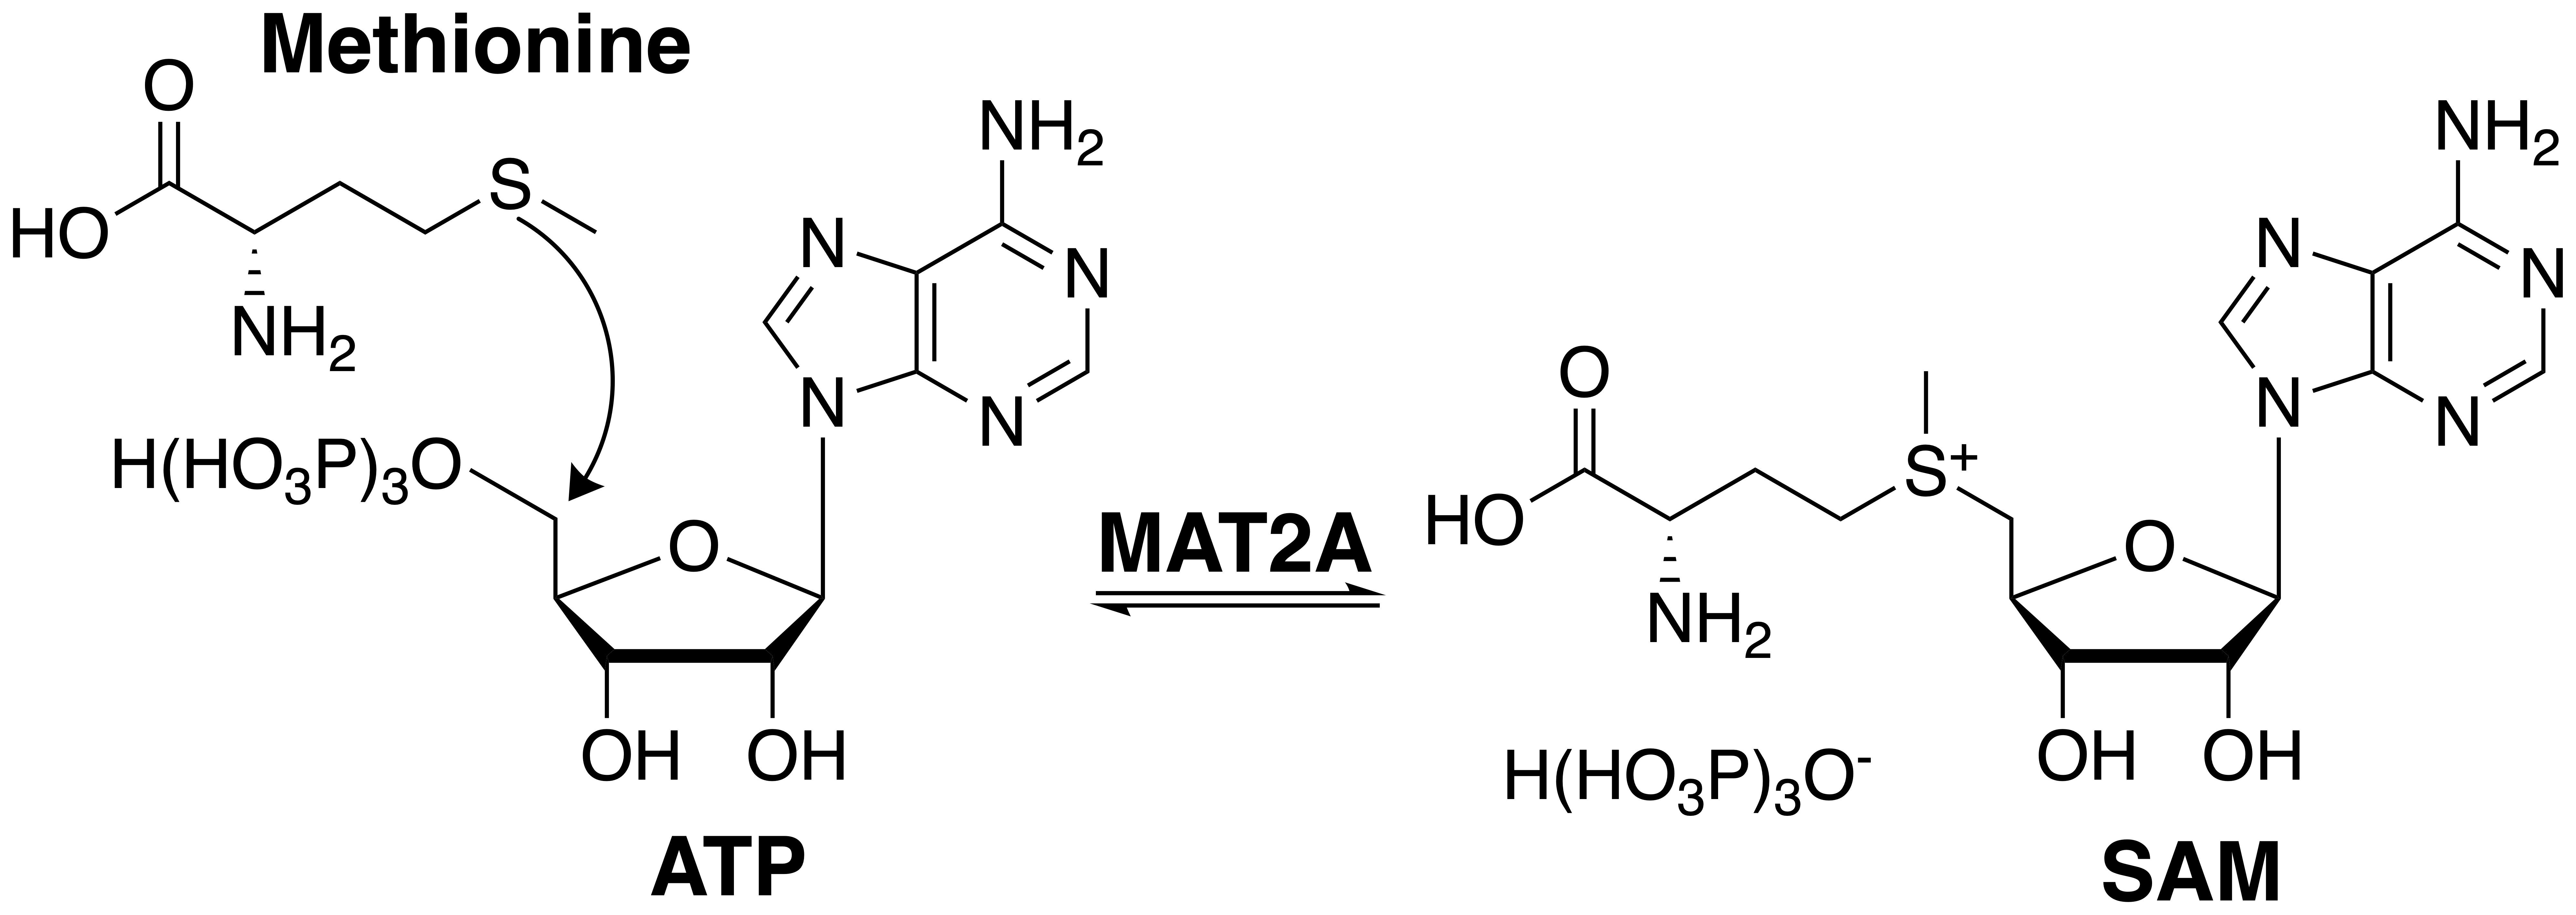
\includegraphics[scale=0.6]{figures/mat2a-reaction.png}
\end{figure}
\end{frame}
%------------------------------------------------------------------------------
\begin{frame}
\frametitle{System preparation}
The energies of both the systems were minimized using 50 steps of the 
steepest descent method, followed by 2000 steps of the
adopted basis Newton-Raphson method where only classical molecular mechanics 
was used for the dynamics. 
The minimized systems were
heated slowly to 300 K for 35 ps beginning with harmonic
constraints on all atoms except on the H atoms and the TIP3P 
water molecules with gradual reduction of the restraint forces. 
15 ps of equilibration was carried out starting with harmonic 
restraint forces followed by 20 ps of constraint free 
equilibration to prepare the systems for TPS simulations. 
During the heating and equilibration steps, bonds that contain 
hydrogen atoms in the MM region were restrained to their equilibrium values 
using the SHAKE procedure. %\cite{Ryckaert77JComputPhys23p327} 
\end{frame}
%------------------------------------------------------------------------------
\begin{frame}
\frametitle{System preparation}
\begin{figure}
\centering 
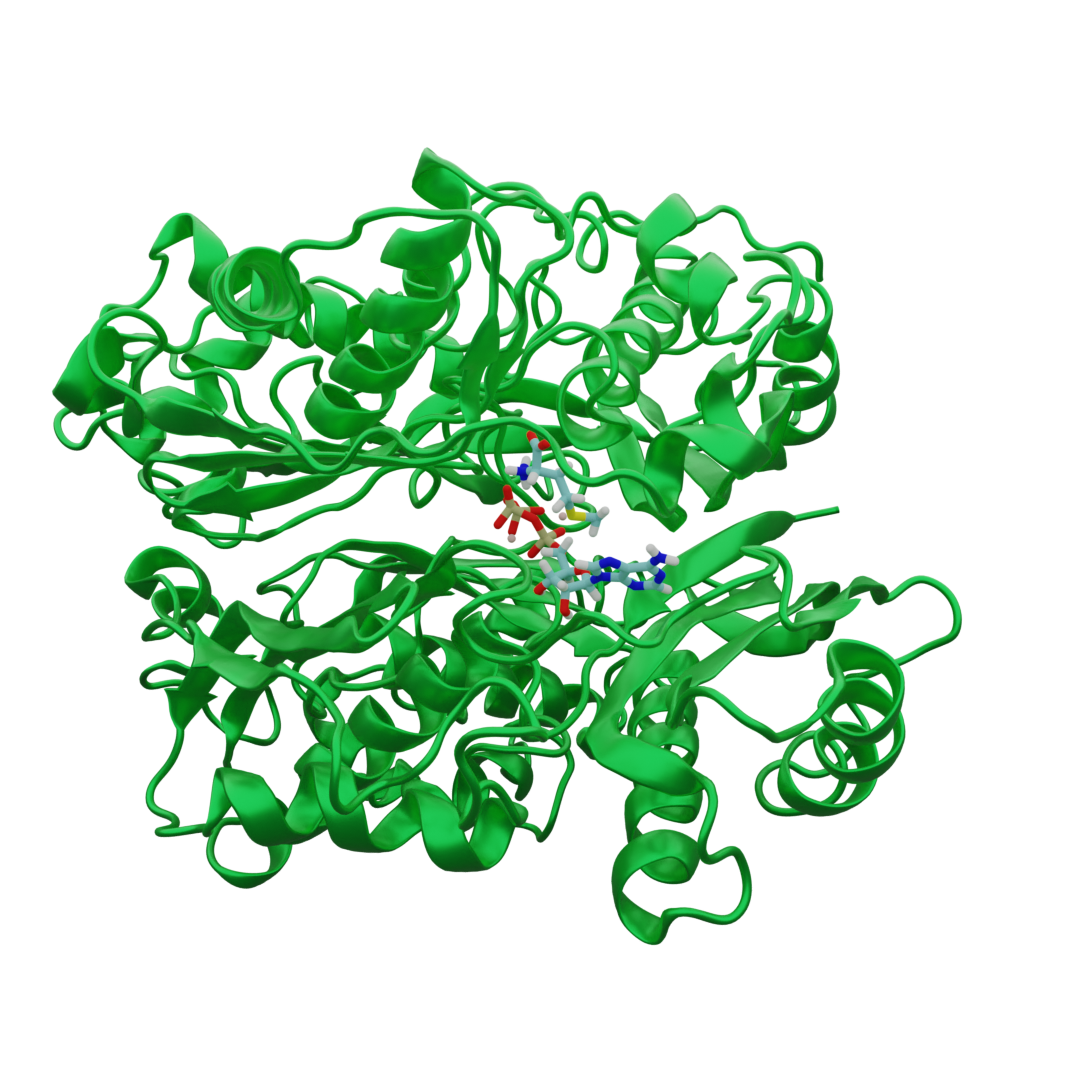
\includegraphics[scale=0.2]{figures/mat2a-equil.png}
\end{figure}
\end{frame}
%------------------------------------------------------------------------------
\begin{frame}
\frametitle{Committor analysis}

\end{frame}
%------------------------------------------------------------------------------
\begin{frame}
\frametitle{Committor distribution analysis}
\begin{figure}[ht!]
\centering
\begin{minipage}[b]{0.45\linewidth}
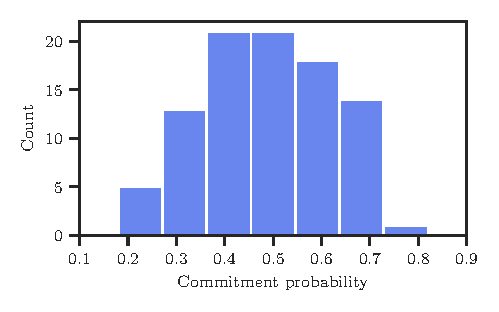
\includegraphics[width=\textwidth]{figures/comm-60-mat2a-nocons.pdf}
\label{fig:minipage1}
\end{minipage}
\quad
\begin{minipage}[b]{0.45\linewidth}
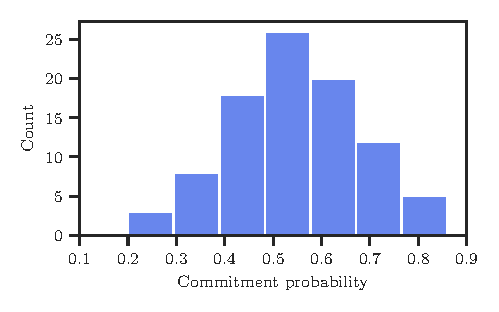
\includegraphics[width=\textwidth]{figures/comm-60-mat2a.pdf}
\label{fig:minipage2}
\end{minipage}
\caption{Committor distribution analysis for obtaining the reaction coordinate of the 
MAT2A catalyzed reaction. The figure on the left has the QM region constrained and the figure 
on the right has the QM region along with the Gln113, Ser114, Arg249 and Arg264 residues constrained.}
\label{fig:mat2a-comm-dist}
\end{figure}
\end{frame}
%------------------------------------------------------------------------------
\begin{frame}
\frametitle{Transition states}
\begin{figure}
\centering
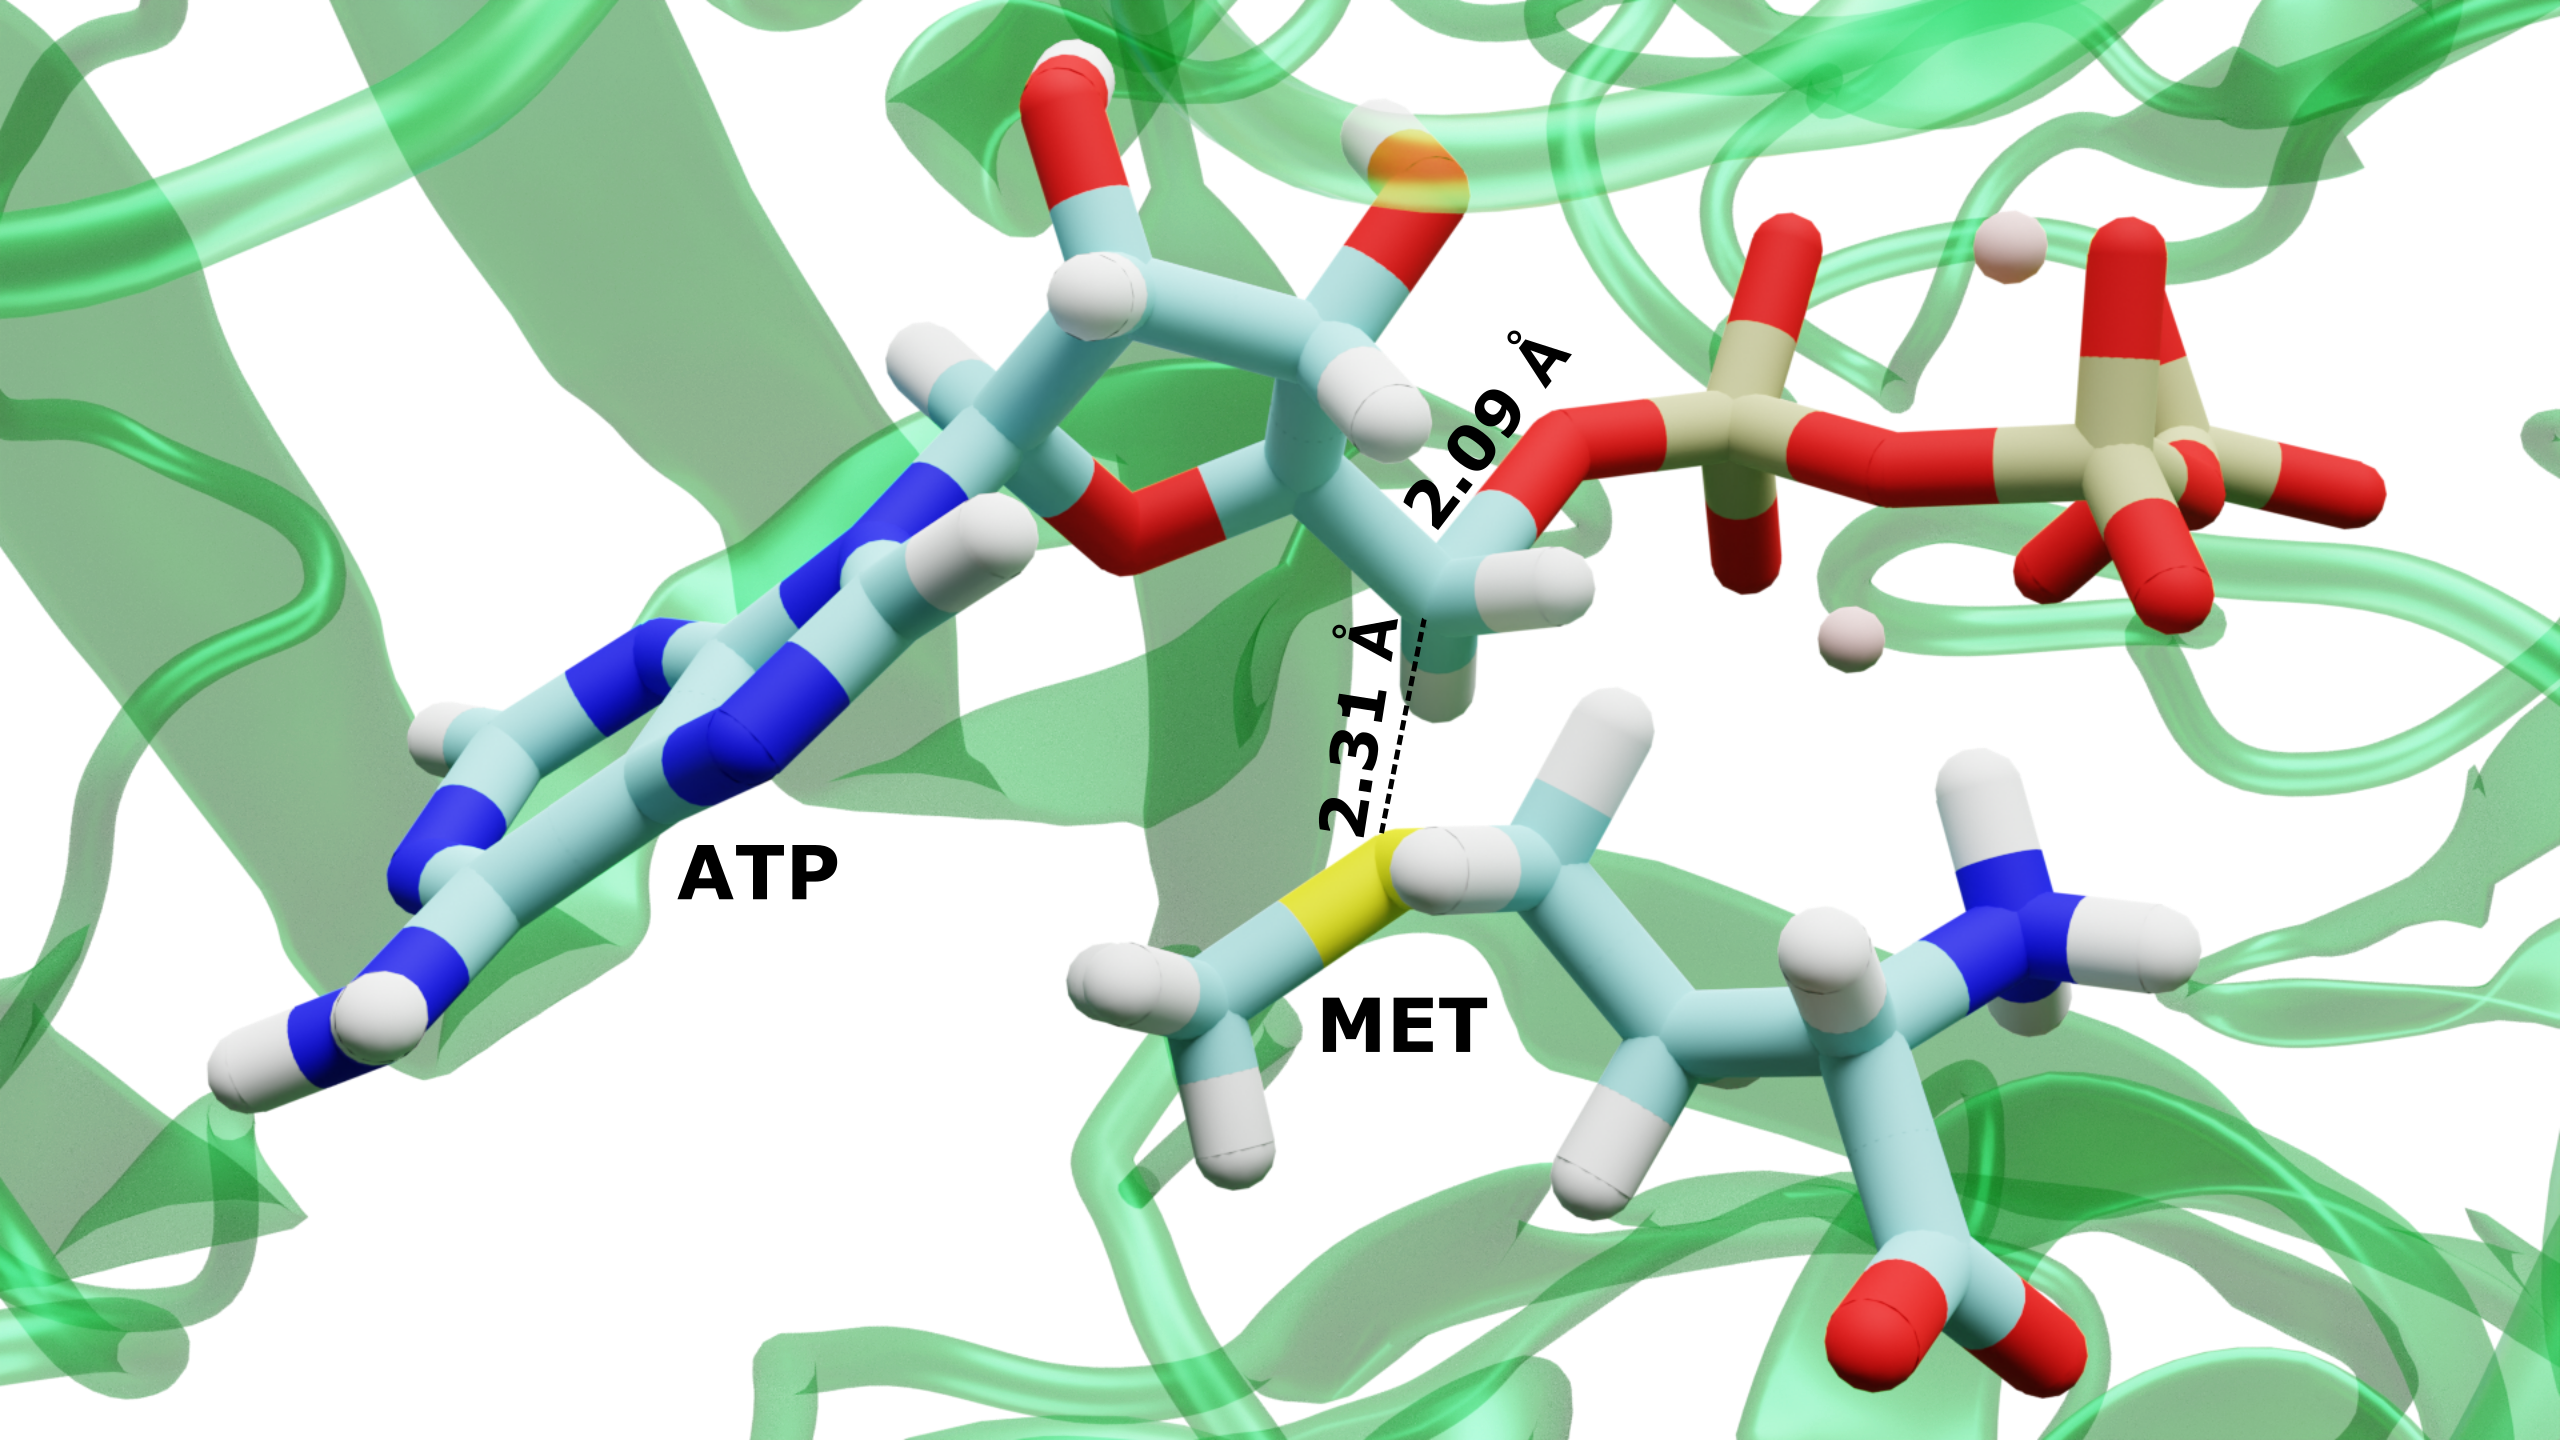
\includegraphics[scale=0.1]{figures/mat2a-trans-labelled.png}
\end{figure}
\end{frame}
%------------------------------------------------------------------------------
\begin{frame}
\frametitle{Free energies}
\begin{figure}
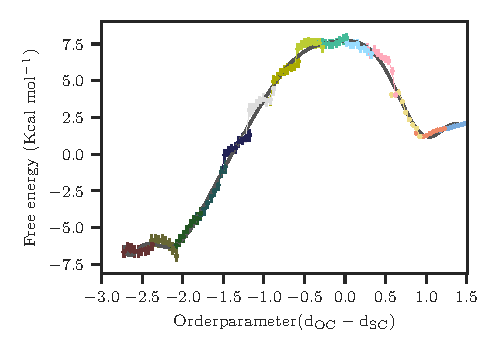
\includegraphics[scale=0.6]{figures/mat2a-fenergy.pdf}
\end{figure}
\end{frame}
%------------------------------------------------------------------------------
\begin{frame}
\frametitle{Plasmodium falciparum adenosine deaminase}
A common drug target to treat malaria.
\begin{figure}
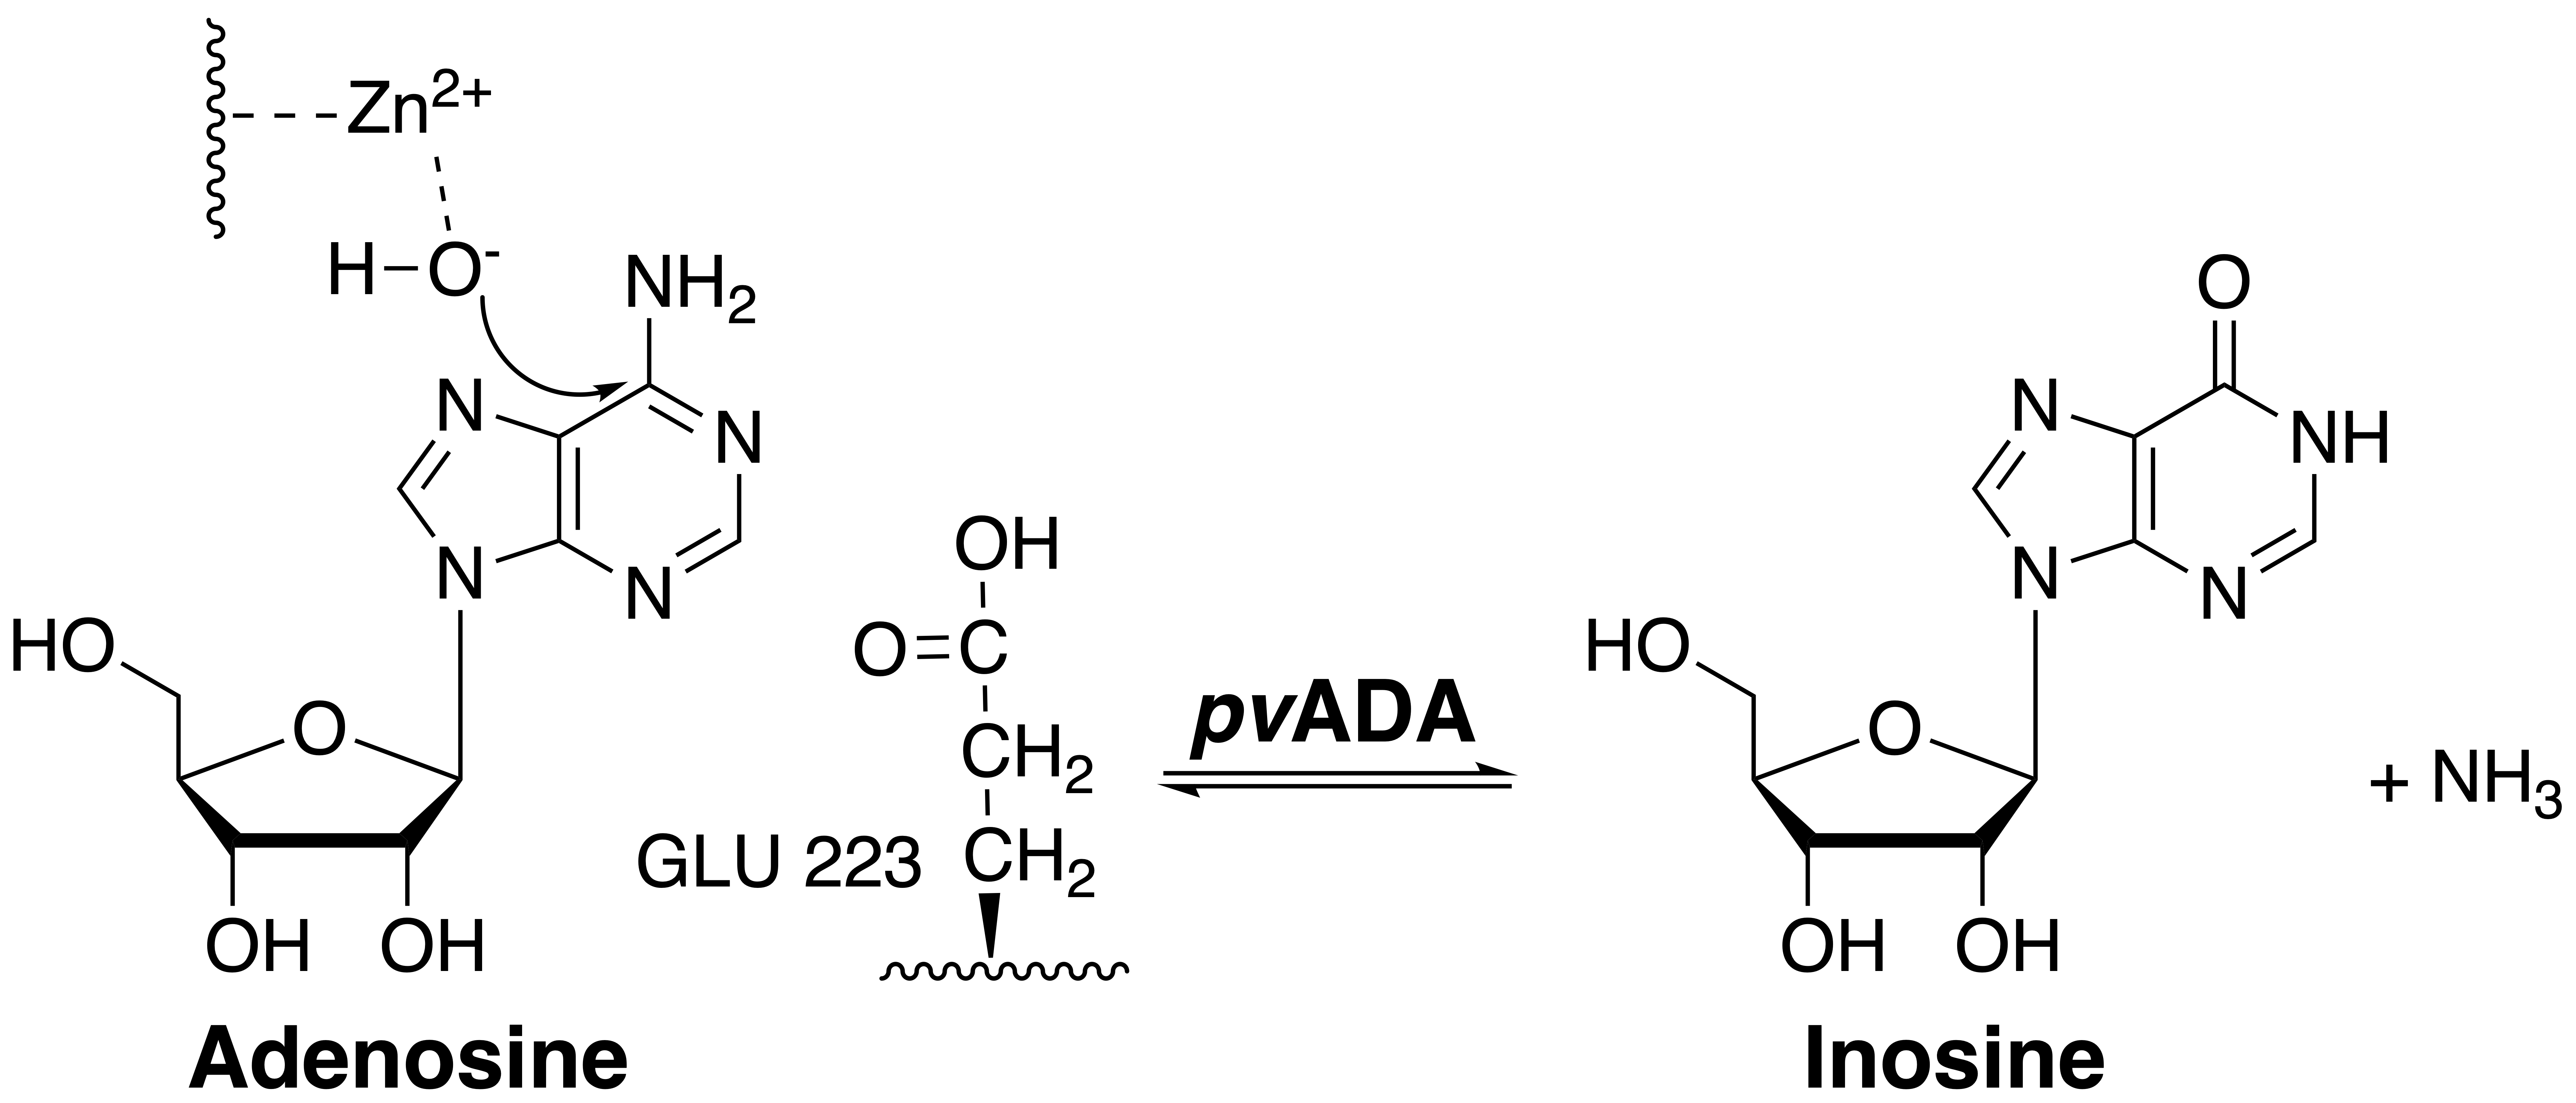
\includegraphics[scale=0.6]{figures/ada-reaction.png}
\end{figure}
\end{frame}
%------------------------------------------------------------------------------
\begin{frame}
\frametitle{Equilibrium structure}
A common drug target to treat malaria.
\begin{figure}
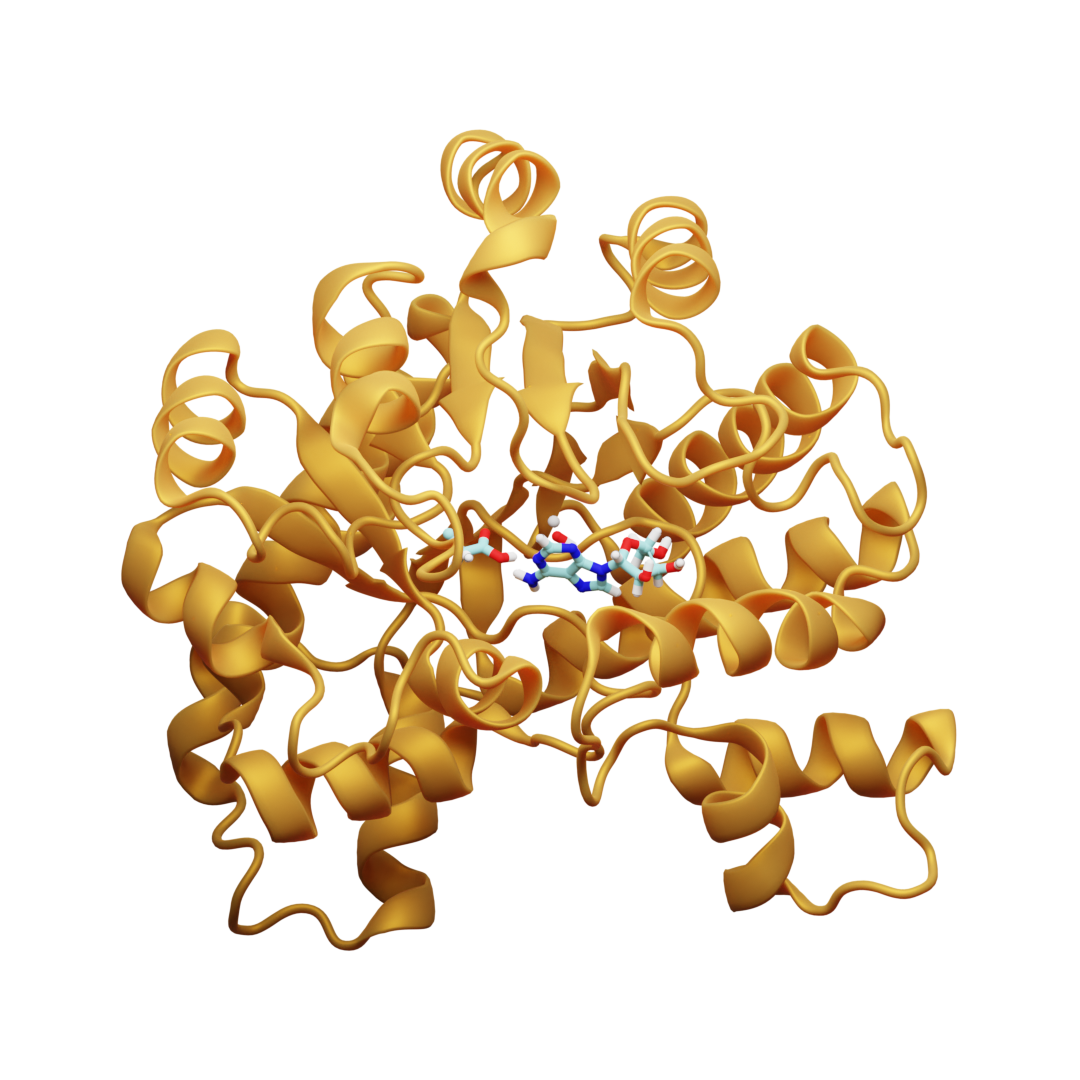
\includegraphics[scale=0.6]{figures/ada-equil.png}
\end{figure}
\end{frame}
%------------------------------------------------------------------------------
\begin{frame}
\frametitle{Conclusions}

\end{frame}
%------------------------------------------------------------------------------
\begin{frame}
\frametitle{Acknowledgements}
\begin{block}{Schwartz group}
\begin{itemize}
    \item Prof. Steven D. Schwartz
    \item Dr. Dimitri Antoniou
    \item Dr. Anthony Boldau
    \item Dr. Allison Smith
    \item Ananya Chakraborthy
    \item Bai Hei
    \item Clara Frost
    \item Dr. Elango Munusamy
\end{itemize}
\end{block}
\pause

\includegraphics[scale=0.1]{figures/nih-logo.png}
\end{frame}
%------------------------------------------------------------------------------
%\input{BeamerIntro.tex}
%\input{BeamerOverlays.tex}
%\input{funmath.tex}
%\input{BeamerConcl.tex}

\end{document}